\documentclass[border=8pt,tikz]{standalone}
\usepackage{tikz}
% Shared TikZ style for Chapter 5 diagrams.
% Inputted by every standalone diagram file.

\usetikzlibrary{
  arrows.meta,
  positioning,
  shapes.geometric,
  shapes.symbols,
  shapes.multipart,
  shapes.misc,
  fit,
  calc,
  backgrounds,
  decorations.pathmorphing,
  decorations.pathreplacing,
  patterns,
  shadows.blur,
}

% ─── Colour palette ──────────────────────────────────────────────
\definecolor{strixBlue}{HTML}{3B7DD8}     % data sources / inputs
\definecolor{strixGreen}{HTML}{22A699}    % processing / workers
\definecolor{strixOrange}{HTML}{E08036}   % storage
\definecolor{strixRed}{HTML}{E04B4B}      % attacker / external threat
\definecolor{strixPurple}{HTML}{6B5DD3}   % frontend / UI
\definecolor{strixGold}{HTML}{F2BE22}     % models / ML
\definecolor{strixGrey}{HTML}{6E7681}     % neutral / labels
\definecolor{strixDark}{HTML}{1F2933}     % titles / borders

% ─── Common node styles ──────────────────────────────────────────
\tikzset{
  >={Latex[width=2mm,length=2.5mm]},
  font=\sffamily\small,
  every node/.style={align=center},
  comp/.style={
    rectangle, rounded corners=2pt, draw=#1, fill=#1!10, very thick,
    text=strixDark, minimum width=22mm, minimum height=8mm,
    inner sep=4pt,
  },
  comp/.default=strixGreen,
  store/.style={
    cylinder, shape border rotate=90, aspect=0.3, draw=strixOrange,
    fill=strixOrange!12, very thick, text=strixDark,
    minimum width=18mm, minimum height=10mm, inner sep=2pt,
  },
  stream/.style={
    rectangle, rounded corners=2pt, draw=strixOrange,
    fill=strixOrange!8, dashed, thick, text=strixDark,
    minimum width=22mm, minimum height=7mm, inner sep=3pt,
    font=\ttfamily\scriptsize,
  },
  source/.style={comp=strixBlue},
  worker/.style={comp=strixGreen},
  model/.style={comp=strixGold},
  ui/.style={comp=strixPurple},
  ext/.style={comp=strixRed},
  title/.style={font=\sffamily\bfseries, text=strixDark},
  edge/.style={->, thick, draw=strixGrey, font=\sffamily\scriptsize\itshape},
  edgeStrong/.style={->, very thick, draw=strixDark, font=\sffamily\scriptsize\bfseries},
  group/.style={
    rectangle, rounded corners=4pt, draw=strixGrey, dashed, thick,
    inner sep=6pt, fill=strixGrey!4,
  },
  badge/.style={
    rectangle, rounded corners=1pt, fill=#1, text=white,
    font=\sffamily\scriptsize\bfseries, inner sep=2pt,
  },
  badge/.default=strixDark,
  port/.style={
    rectangle, rounded corners=1pt, draw=strixDark, fill=strixGrey!8,
    font=\ttfamily\scriptsize, minimum width=14mm, inner sep=2pt,
  },
}


\begin{document}
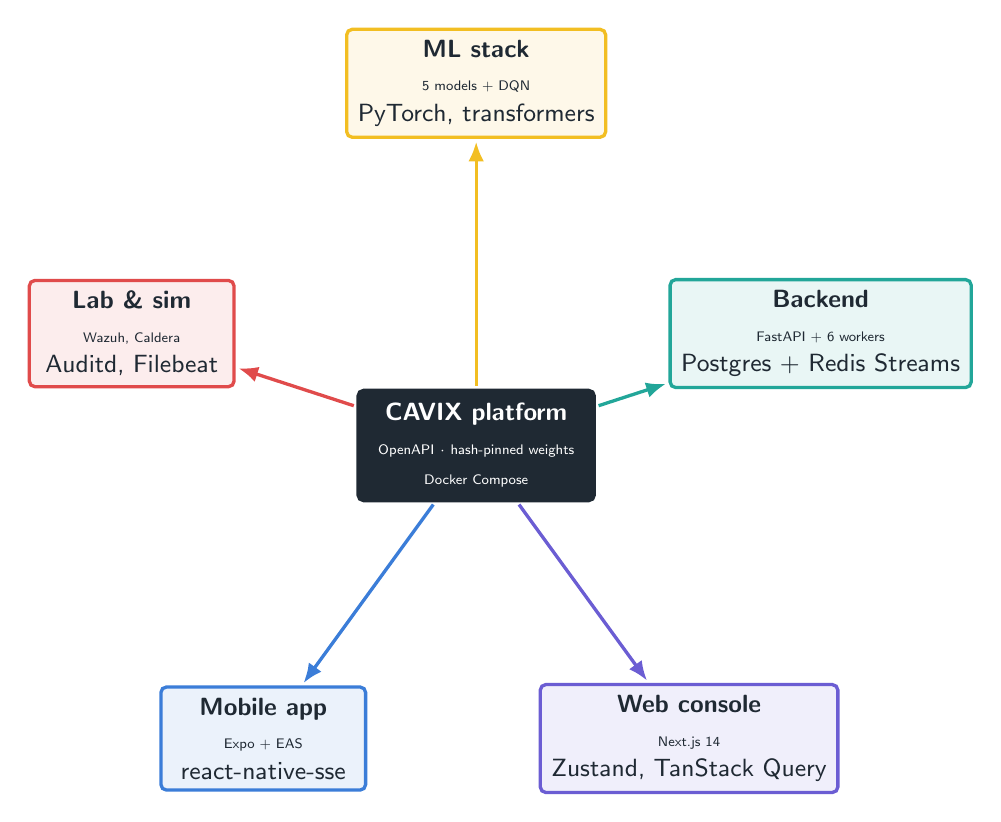
\begin{tikzpicture}[node distance=8mm]

% Central CAVIX hub
\node[comp=strixDark, minimum width=30mm, minimum height=14mm,
      fill=strixDark, text=white, font=\sffamily\bfseries\small]
  (hub) {CAVIX platform\\[1pt]\tiny\mdseries
         OpenAPI \(\cdot\) hash-pinned weights\\\tiny\mdseries Docker Compose};

% Five pillars
\def\R{4.6}
\foreach \i/\name/\sub/\col in {
  0/{ML stack}/{5 models + DQN\\PyTorch, transformers}/strixGold,
  1/{Backend}/{FastAPI + 6 workers\\Postgres + Redis Streams}/strixGreen,
  2/{Web console}/{Next.js 14\\Zustand, TanStack Query}/strixPurple,
  3/{Mobile app}/{Expo + EAS\\react-native-sse}/strixBlue,
  4/{Lab \& sim}/{Wazuh, Caldera\\Auditd, Filebeat}/strixRed%
} {
  \pgfmathsetmacro{\angle}{90 - \i*72}
  \node[comp=\col, minimum width=26mm, minimum height=12mm, font=\sffamily\small]
    at ({\R*cos(\angle)}, {\R*sin(\angle)}) (p\i)
    {\textbf{\name}\\[1pt]\tiny\sub};
  \draw[edgeStrong, draw=\col, shorten >=1pt, shorten <=1pt] (hub) -- (p\i);
}

\end{tikzpicture}
\end{document}
